\section{Introduction} \label{introduction}
In recent years the recognition of handwritten digits has been systematically improved. Benchmarked on the MNIST (Mixed National Institute of Standards and Technology)
dataset that contains about 70.000 images of handwritten digits along with their corresponding labels, numerous papers were published that apply convolutional neural networks (CNNs)
to achieve error rates of 0.23\% \cite{MNIST_2012} or even 0.21\% \cite{MNIST_boosting}.

As these results almost cope with human performance and a good dataset does need to represent a sufficiently challenging problem to stay useful and to ensure its longevity, various adjustments can be contemplated. One way could be the extension of the underlying dataset \cite{EMNIST}.

Another approach would be the extension of the task itself by not only recognizing single digits but whole digit strings. In 2014 the ICFHR (International Conference on Frontiers in Handwriting Recognition) announced a competition to attend that matter: Handwritten Digit String Recognition in Challenging Datasets (HDSRC2014) \cite{icfhr_competition}.

In course of that they proposed a new benchmark framework that consists of two real world datasets and respective evaluation measures. The task's complexity is not only founded on the connected digits but also on the additional challenges that come along with the images' real world nature as document layout, background texture or noisy strokes. 

Traditional approaches to digit string recognition often used segmentation. The string image is segmented to pieces that in best case represent single digits. The recognition results of these single pieces are then combined to get global optimal results. Since these approaches in practice suffer from various handwritten styles, connected or even overlapped characters and noises, \cite{zhan2017} proposes an segmentation free approach. 

Their model uses ResNet with convolutional layers \cite{ResNet} as an discriminative sequence extractor and feature decoder, combines it with an bidirectional LSTM and calculates the loss with connectionist temporal classificiation (CTC) \cite{CTC}.

Since this approach achieved remarkable results on the given datasets we used it as fundament for our own model.

The rest of this paper is organized as follows. In Section 2 we briefly describe the real world datasets given by the HDSRC2014. ...... Then, details of our experiments are presented in Section 3. Section 4 concludes this paper and discusses potential future work.

\section{Databases} \label{Datasets}
There are two different databases for recognizing handwritten digit strings we used in our experiments.

The first database, named ORAND-CAR, is a real world database with 11719 images of the 'Courtesy Amount Recognition (CAR)' field of bank checks. It originates from two different sources, one bank of Chile and one of Uruguay, and therefore shows different characteristics in terms of check layout, image quality and further noise. That is the reason the database is splitted into two subsets called ORAND-CAR-A (CAR-A) and ORAND-CAR-B (CAR-B). Samples of both datasets are shown in Figure \ref{fig:carA} and \ref{fig:carB}.

\begin{figure}
  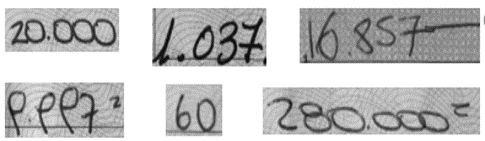
\includegraphics[width=\linewidth]{images/CAR-A-Splitted.png}
  \caption{\it Sample images of ORAND-CAR-A}
  \label{fig:carA}
\end{figure}

\begin{figure}
  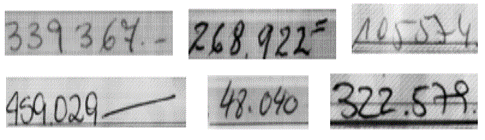
\includegraphics[width=\linewidth]{images/CAR-B-Splitted.png}
  \caption{\it Sample images of ORAND-CAR-B}
  \label{fig:carB}
\end{figure}

CAR-A's training set consists of 2009 images whereas the testing set delivers 3784 images. In CAR-B there are 3000 training images and 2926 images for testing.

The second database we worked on is called Computer Vision Lab Handwritten Digit String (CVL HDS). It contains handwritten digits of 300 different writers without any background noise. The training set includes only 10 different digit strings from about 125 writers which leads to an overall amount of 1262 images for training. In the testing set we have the same 10 digit strings from the remaining writers and 16 new strings from all 300 writers to reach 6698 testing images. CVL HDS provides us with large variability with respect to handwriting styles but lacks diversity in the digit strings themselves. Examples of the CVL HDS database are shown in Figure \ref{fig:cvl}.

\begin{figure}
  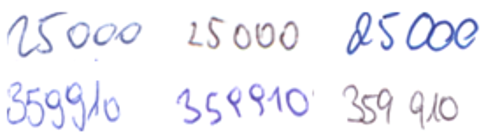
\includegraphics[width=\linewidth]{images/CVL-HDS-Splitted.png}
  \caption{\it Sample images of CVL HDS}
  \label{fig:cvl}
\end{figure}

The datasets differ with respect to their string lengths. CVL has images with string lengths from 5 to 7 whereas CAR-B offers digit strings from length 4 to 8. In this regard CAR-A comes with the biggest variety and covers a string length range from 2 to 8 digits. A summary of the string length distribution can be seen in Table \ref{table_string_lengths}.

\begin{table}
\caption{\label{table_string_lengths} {\it Summary of string length distribution.}}
\vspace{2mm}
\hspace{1mm}
\begin{adjustbox}{width=0.45\textwidth}
\centerline{
\begin{tabular}{|l|lll|lll|}
\hline
\multicolumn{1}{|l|}{} & & Training & & & Testing & \multicolumn{1}{l|}{}\\
\multicolumn{1}{|l|}{len} & \multicolumn{1}{l|}{CAR-A} & \multicolumn{1}{l|}{CAR-B} & \multicolumn{1}{l|}{CVL} & \multicolumn{1}{l|}{CAR-A} & \multicolumn{1}{l|}{CAR-B} & \multicolumn{1}{l|}{CVL} \\ \hline \hline
2 & 22 & 0 & 0 & 36 & 0 & 0  \\
3 & 204 & 0 & 0 & 387 & 5 & 0  \\
4 & 704 & 63 & 0 & 1425 & 69 & 0  \\
5 & 903 & 1200 & 125 & 1475 & 1241 & 789  \\
6 & 145 & 1599 & 758 & 363 & 1452 & 4144  \\
7 & 29 & 137 & 379 & 87 & 157 & 1765  \\
8 & 2 & 1 & 0 & 11 & 2 & 0  \\
\hline
$\Sigma$ & 2009 & 3000 & 1262 & 3784 & 2926 & 6698  \\
\hline
\end{tabular}}
\end{adjustbox}
\end{table}

Since the images of the used databases come in lots of different aspect ratios and we want them to fit our model, we resize them to a fixed width of 120 and an height of 50.

 We furthermore make use of the different tools given by Pytorch to augment our data. Dynamic data augmentation is achieved with help of the functions ColorJitter() and RandomAffine(). How the data is transformed, can be seen in Figure \ref{fig:dataAug}.

\begin{figure}
  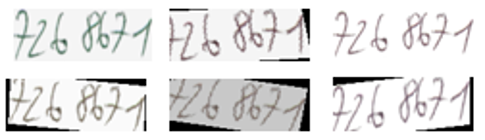
\includegraphics[width=\linewidth]{images/Data-Augmentation.png}
  \caption{Examples of an image after preprocessing and data augmentation.}
  \label{fig:dataAug}
\end{figure}